
\documentclass{beamer}

\usepackage{algpseudocode}

\usetheme{Montpellier}
\usecolortheme{rose}

% page numbers, from
% https://tex.stackexchange.com/questions/137022/how-to-insert-page-number-in-beamer-navigation-symbols
\expandafter\def\expandafter\insertshorttitle\expandafter{%
  \insertshorttitle\hfill%
  \insertframenumber\,/\,\inserttotalframenumber}

\newcommand{\stanza}{ \\~\ }

\title{02. Algorithm Fundamentals}
\subtitle{CPSC 535 $\sim$ Fall 2019}
\author{Kevin A. Wortman}
\institute{ 
\includegraphics[height=2cm]{csuf-logo-cmyk} }
\date{August 28, 2019 \stanza

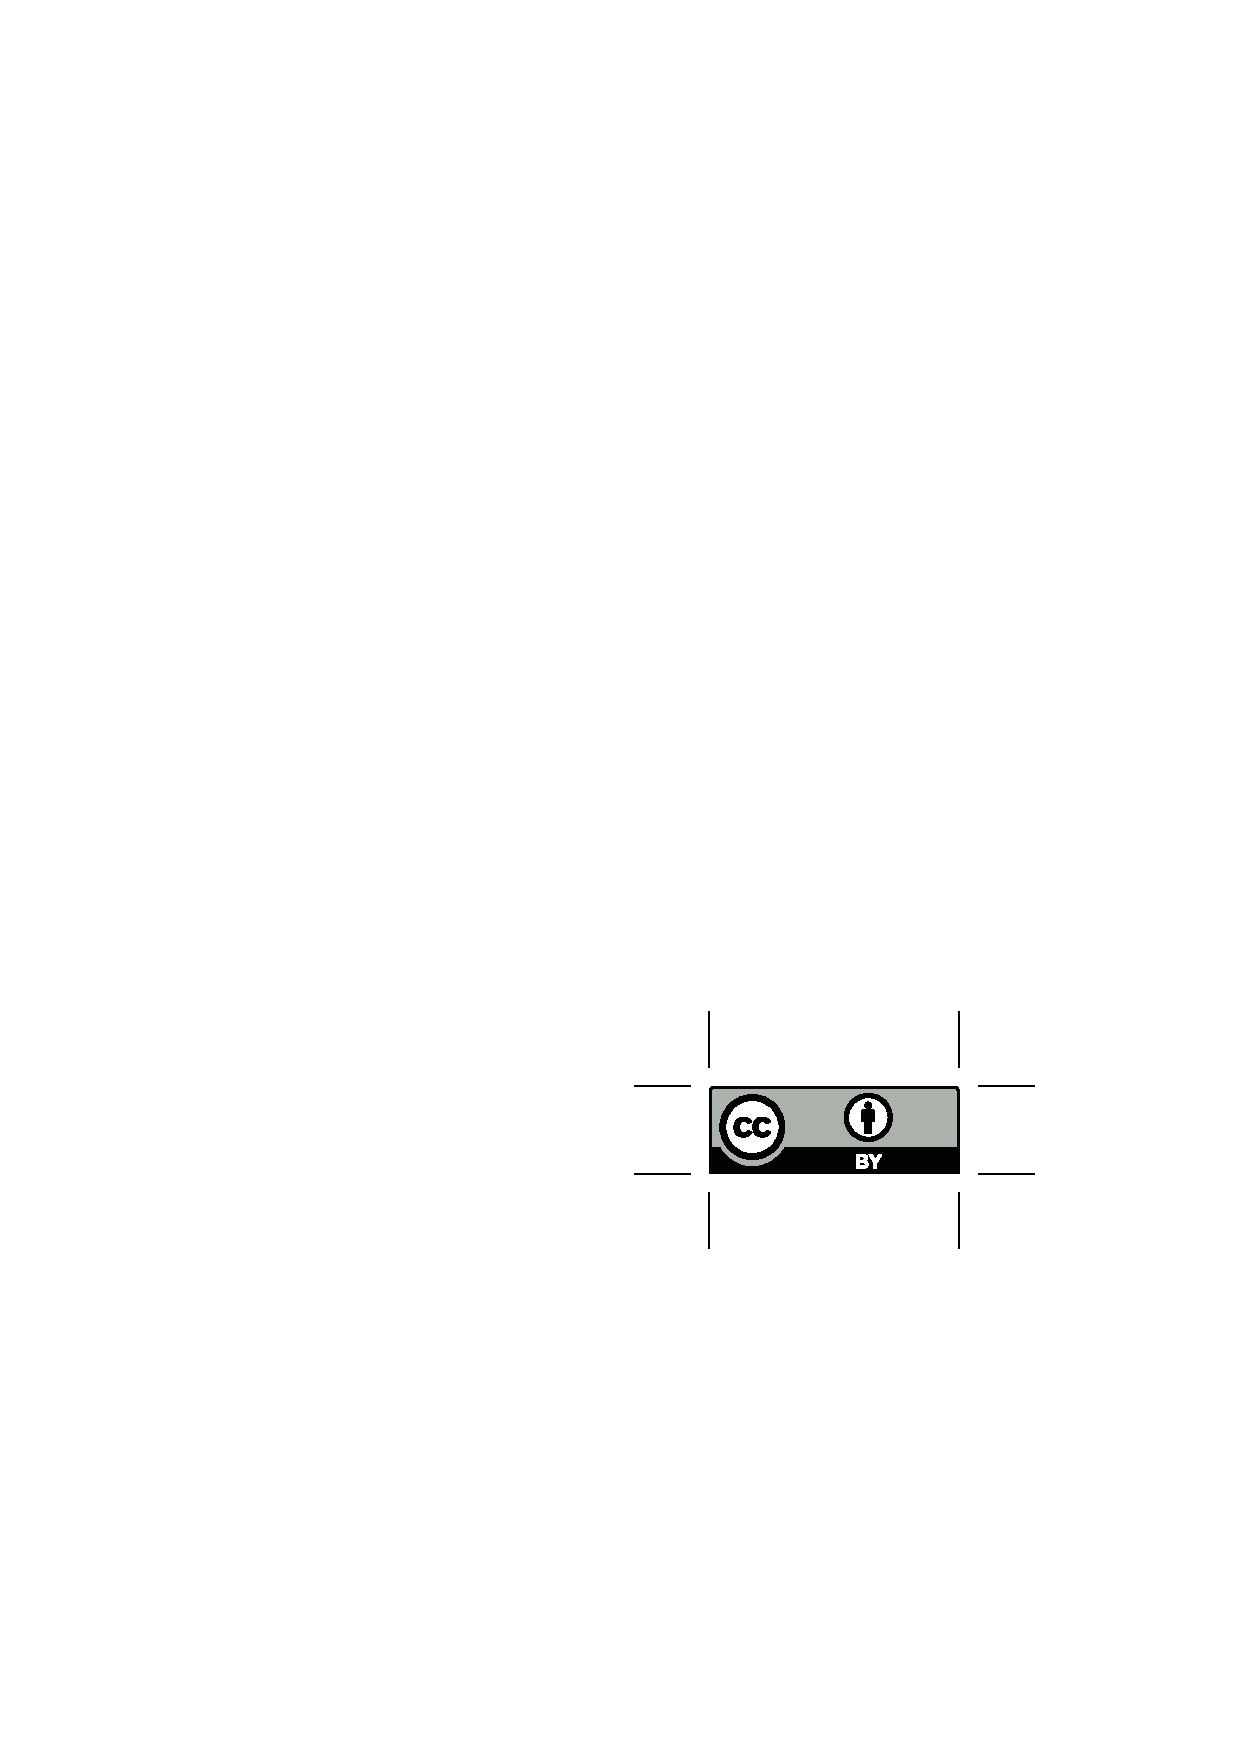
\includegraphics[height=14pt]{by} \\

{\tiny
This work is licensed under a
\href{http://creativecommons.org/licenses/by/4.0/}{Creative Commons Attribution 4.0 International License}.
}}

\begin{document}

\begin{frame}
  \titlepage
\end{frame}

\begin{frame} \frametitle{Problems}

  \emph{Computational problem:} definition of input and desired output \stanza

  Each is a mathematical object that could be stored in a computer data
  structure.  \stanza

  \emph{\textbf{Sorting problem}} \\
  \textbf{input:} A sequence of $n$ numbers
    $\langle a_1, a_2, \ldots, a_n \rangle.$ \\
  \textbf{output:} A permutation (reordering)
    $\langle a_1', a_2', \ldots, a_n' \rangle$ of the input sequence such
    that $a_1' \le a_2' \le \ldots \le a_n'.$
\end{frame}

\begin{frame} \frametitle{Algorithms}
  \emph{Instance (of a problem):} Concrete input datum \stanza

  \begin{example}
    $\langle 71, 14, 31, 2, 82 \rangle$
  \end{example}

  \emph{Algorithm:} well-defined computational procedure that unerringly
    transforms input to output
\end{frame}

\begin{frame} \frametitle{Motivation}
  Why do we care about algorithms, or algorithmic efficiency?
  \begin{itemize}
    \item Algorithms are automating major parts of the economy: operations
      research, high frequency trading, machine learning, etc.
    \item Efficiency can mean the difference between computations being
      viable, sustainable, for human use versus impractical.
    \item The principle of not wasting product.
    \item Intriguing mathematical questions are worth studying in their own
      right.
  \end{itemize}
\end{frame}

\begin{frame} \frametitle{Data Structures}
  \emph{Data Structure:} method for storing, organizing data
  \begin{itemize}
    \item Data members e.g. head pointer, tail pointer
    \item \emph{Invariant(s)} defining how the structure must be organized
      to remain valid, e.g. head points to first node, tail points to last node
    \item Defined \emph{operations,} each operation is an algorithm that
      operates on the structure.
    \end{itemize}
\end{frame}

\begin{frame} \frametitle{Pseudocode}
  \emph{Pseudocode:} code-like notation for conveying algorithms
  \begin{itemize}
    \item Goal is clear communication to a human audience
    \item Not compiled, so no need to be syntactically perfect
    \item Not software engineering; no need for error checking, modularity,
      encapsulation, etc. \stanza
  \end{itemize}

  \emph{Algorithm implementer} is a specific role and skill set, bridging the
    gap between scholarly pseudocode and industrial coding practices.
\end{frame}

\begin{frame} \frametitle{Insertion Sort}

\begin{algorithmic}[1]
  \Function{INSERTION-SORT}{A}
  \For{j = 2 to A.length}
    \State key = A[j]
    \State // Insert A[j] into the sorted sequence A[1 \ldots j-1].
    \State i = j - 1
    \While{$i > 0$ and $A[i] > key$}
      \State A[i+1] = A[i]
      \State i = i-1
    \EndWhile
    \State A[i+1] = key
  \EndFor
  \EndFunction
\end{algorithmic}

\end{frame}

\begin{frame} \frametitle{Pseudocode Observations}
  \begin{itemize}
    \item Algorithm is a function/procedure, input is argument(s)
    \item No global variables
    \item Code-like but not compile-able code
    \item Arrays start at 1
    \item No error checking or modularity
    \item Translatable into practically any programming language
  \end{itemize}
\end{frame}

\begin{frame} \frametitle{Analysis}
  \emph{Analysis:} establish how efficient an algorithm is
  \begin{itemize}
    \item Usually a mathematical proof (alternatively empirical evidence)
    \item Usually analyze for time spent (or disk I/O, space, energy,
      randomness, etc.)
    \item Usually summarize resource use by \emph{order of growth} in
      asymptotic notation; $O(n), \Theta(n^2)$, etc.
  \end{itemize}
\end{frame}

\begin{frame} \frametitle{RAM model}
  \emph{Computational model:} defines how a computer executes an algorithm,
    specifically enough to measure time (or other resources)

  \emph{Random Access Machine (RAM):}
  \begin{itemize}
    \item "default" computational model, approximates a generic real-world
      CPU and memory
    \item CPU has instructions for integer arithmetic, floating point arithmetic,
      control (jump, call, return, if), logic (or, and, not), data copying.
    \item one step $\equiv O(1)$ instructions; each pseudocode statement counts
      as 1 step (except function calls)
    \item CPU has some $O(1)$ word size, e.g. 32 or 64 bit; one instruction
      is limited to writing that many bits
    \item cannot "cheat" by packing $\Theta(n)$ information in one word
  \end{itemize}
\end{frame}

\begin{frame} \frametitle{Worst-Case Analysis}
  \begin{itemize}
  \item In a time analysis, we need to prove how much time insertion sort
    takes when run
  \item depends on the type of input, e.g. pre-sorted, completely jumbled,
    in between
  \item convention: analyze the \emph{worst case} for the algorithm at hand
  \item generous to skeptics, conservative for software engineers
  \item as an exception, sometimes analyze \emph{average case} of
    deliberately randomized algorithms
  \end{itemize}

  \emph{Claim:} The worst-case time complexity of insertion sort is
    $\Theta(n^2).$

\end{frame}

\begin{frame} \frametitle{Divide-and-conquer}
  \begin{enumerate}
    \item \textbf{divide} input into several smaller instances of the same
      problem (often, divide input in half)
    \item \textbf{"conquer"} by recursively solving all the sub-problems;
      may involve a simple base case
    \item \textbf{combine} the many solutions into one coherent solution for
      the original problem
  \end{enumerate}
\end{frame}

\begin{frame} \frametitle{Merge sort}
  \emph{Merge sort:} classical sorting algorithm using divide-and-conquer \stanza

  \textbf{divide:} chop list of $n$ unsorted elements into two lists of $n/2$
    elements each

  \textbf{conquer:} merge-sort each unsorted list; if $n \leq 1,$ nothing to do

  \textbf{combine:} \emph{merge} two sorted lists of $n/2$ elements, into one
    sorted list of $n$ elements

\end{frame}

\begin{frame} \frametitle{Merge pseudocode}

  \begin{columns}
  \begin{column}{0.4\textwidth}
    {\tiny
      \begin{algorithmic}[1]
        \Ensure $A[p \ldots r]$ is sorted
        \Function{MERGE-SORT}{A, p, r}
        \If{$p < r$}
          \State $q = \lfloor (p+r) / 2 \rfloor$
          \State MERGE-SORT($A, p, q$)
          \State MERGE-SORT($A, q+1, r$)
          \State MERGE($A, p, q, r$)
        \EndIf
        \EndFunction
      \end{algorithmic}
    }
\end{column}
\begin{column}{0.6\textwidth}

    {\tiny
    \begin{algorithmic}[1]
      \Require $p \leq q < r$, $A[p \ldots q]$ is sorted, $A[q+1 \ldots r$] is sorted
      \Ensure $A[p \ldots r]$ is sorted
      \Function{MERGE}{A, p, q, r}
      \State $n_1 = (q-p+1), \, n_2 = (r-q)$
      \State let $L[1 \ldots n_1+1]$ and $R[1 \ldots n_2 + 1]$ be new arrays
      \State $L[1 \ldots n_1] = A[p \ldots q]$
      \State $R[1 \ldots n_2] = A[p+1 \ldots q]$
      \State $L[n_1+1] = R[n_2+2] = \infty$
      \State $i = j = 1$
      \For{$k=p$ to $r$}
          \If{$L[i] \leq R[j]$}
              \State $A[k] = L[i]$
              \State $i = i + 1$
          \Else
              \State $A[k] = R[j]$
              \State $j = j + 1$
          \EndIf
      \EndFor
      \EndFunction
    \end{algorithmic}
    }

\end{column}
\end{columns}
\end{frame}

\begin{frame} \frametitle{Merge sort analysis}
  The worst-case time complexity of merge sort is given by the
  \emph{recurrence relation}

  \begin{equation*}
    T(n) = \begin{cases}
            \Theta(1) & \text{ if } n=1, \\
            2 T(n/2) + \Theta(n) & \text{ if } n > 1 .
          \end{cases}
  \end{equation*}

  \emph{Claim:} $T \in \Theta(n \log n)$ \stanza

  \emph{Claim:} Merge sort uses $\Theta(n)$ extra space for $L$ and $R.$
  (Observe that at most one merge is happening at any moment, and the largest
   merge uses $n+2$ extra array elements.)
\end{frame}

\begin{frame} \frametitle{Insertion sort versus merge sort}
  Insertion sort: $\Theta(n^2)$ time, $\Theta(1)$ space \stanza

  Merge sort: $\Theta(n \log n)$ time, $\Theta(n)$ space \stanza

  Merge sort is subjectively more convoluted \stanza

  Space vs. time tradeoff (typical) \stanza

  Efficiency vs. convolution tradeoff (typical) \stanza

  Refactoring convolution into algorithm design is usually a win

\end{frame}

\begin{frame} \frametitle{Asymptotic notation}
\emph{Asymptotic notation:} $\Theta(n^2), O(n^2), \Omega(n^2),$ etc. \stanza

Solves some problems with algorithm analysis
\begin{itemize}
  \item Whole point is how algorithms perform on very large $n$
  \item $\implies$ ignore small $n$
  \item We count abstract "steps" so constant factors are not meaningful
  \item i.e. $4n^2$ and $5n^2$ should count as essentially the same
  \item Want to prioritize speeding up the part of the algorithm that actually
    accounts for the most time
  \item Running time functions usually include multiple terms; the
    asymptotically fastest-growing term \emph{dominates} the running time
\end{itemize}
\end{frame}

\begin{frame} \frametitle{Example: insertion sort}

Suppose insertion sort's run time is
\begin{align*}
  T(n) &= \text{(inner loop steps)} + \text{(outer loop steps)} + \text{(outside loop)} \\
  &= 3n^2 + 4n + 1 \\
\end{align*}

Let $n=2,$
\[ T(n) = 3(2)^2 + 4(2) + 1 = 12 + 8 + 1 = 21 .\]

Let $n=1,000,$
\[ T(n) = 3(1,000)^2 + 4(1,000) + 1 = 3,000,000 + 4,000 + 1 . \]

$\implies$ inner loop dominates time, focus on speeding that up

\end{frame}

\begin{frame} \frametitle{$\Theta$ notation}
"big-theta": intuitively,
\[ \Theta(g(n)) = \{ f(n) \,:\, f(n)
  \text{ grows asymptotically the same as } g(n) \} \]

Formally,
\begin{align*}
  \Theta(g(n)) = \{ f(n) :\, & \exists \text{ positive constants } c_1, c_2, n_0 \\
   & \text{ such that } 0 \leq c_1 g(n) \leq f(n) \leq c_2 g(n)
   & \forall n \geq n_0 \} .
\end{align*}

This is set notation, so e.g.
\[ 3n^2 + 4n + 1 \in \Theta(n^2) . \]

$\Theta$-notation indicates a \emph{tight bound:} set of functions upper-
\textbf{and} lower-bounded by $g(n)$

\end{frame}

\begin{frame} \frametitle{$O, \Omega, o, \text{ and } \omega$}
Intuitively,
\begin{itemize}
  \item "big-oh": \[ O(g(n)) = \{ f(n) \,:\, f(n)
    \text{ grows asymptotically } \leq  g(n) \} \]
  \item "big-omega": \[ \Omega(g(n)) = \{ f(n) \,:\, f(n)
    \text{ grows asymptotically } \geq  g(n) \} \]
  \item "little-oh": \[ o(g(n)) = \{ f(n) \,:\, f(n)
    \text{ grows asymptotically } <  g(n) \} \]
  \item "little-omega": \[ \omega(g(n)) = \{ f(n) \,:\, f(n)
    \text{ grows asymptotically } >  g(n) \} \]
 \end{itemize}
\end{frame}

\begin{frame} \frametitle{Knuth-style notation abuse}

  An asymptotic notation expression such a $O(n^2)$ is, technically, a
  \textbf{set} of function objects \stanza

  $\implies$ a run-time function may be an \textbf{element} of one of these sets \stanza

  Mathematically precise: \[ 3n^2+4n+1 \in O(n^2). \]

  Some others (notably Knuth) abuse notation to use $=$, which is technically incorrect
  since the operands are different types, but is arguably more readable:
  \[ 3n^2 + 4n +1 = O(n^2) .\]

\end{frame}

\end{document}
